% Course-compliant layout; restrained title rules and headings inspired by NeurIPS.
% Compile from this directory with pdflatex (twice). No external bibliography needed.
\documentclass[11pt,letterpaper]{article}
\usepackage[T1]{fontenc}
\usepackage[utf8]{inputenc}
\usepackage{lmodern}
\usepackage[margin=1in]{geometry}
\usepackage{microtype,amsmath,booktabs,graphicx,float,enumitem}
\usepackage[font=normalsize,labelfont=bf,skip=3pt]{caption}
\usepackage{titlesec}
\usepackage[numbers,sort&compress]{natbib}
\usepackage[hidelinks]{hyperref}
\hypersetup{pdftitle={Privacy-Fairness Trade-offs in DP-SGD: ECE 285 Progress Report},pdfauthor={Cici Xu and Shannon Saad}}
\linespread{1}
\setlength{\parindent}{0pt}
\setlength{\parskip}{3pt}
\setlength{\intextsep}{5pt}
\titleformat{\section}{\normalfont\normalsize\bfseries}{\thesection}{0.5em}{}
\titlespacing*{\section}{0pt}{6pt}{2pt}
\newcommand{\eps}{\varepsilon}
\begin{document}
\begin{center}
\hrule height 1pt\vspace{4pt}
{\large\bfseries Privacy--Fairness Trade-offs in DP-SGD}\par
\vspace{3pt}
Cici Xu \qquad Shannon Saad\par
ECE 285 Progress Report \quad November 18, 2026
\vspace{4pt}\hrule height 0.5pt
\end{center}
\vspace{-4pt}

\section{Introduction and Project Objectives}
We extend Bagdasaryan et al.'s unequal privacy-cost analysis~\cite{bagdasaryan2019} to Folktables
employment prediction~\cite{ding2021}. We ask whether DP-SGD disproportionately reduces group accuracy,
how privacy budgets affect accuracy/fairness, and whether Learning Fair Representations
(LFR)~\cite{zemel2013} and equalized-odds (EO) post-processing~\cite{hardt2016} mitigate disparities.

\section{Progress Since Proposal}
The instructor's feedback was positive and encouraged \textbf{additional Folktables tasks}.
ACSIncome is planned; only employment experiments are complete.
Independent refinements add sex/race predictors (primary), exclusion (sensitivity), five-seed comparisons,
and sampling/clipping controls. Data preparation and baseline/DP experiments are complete; LFR/EO are planned.

\section{Experimental Setup and Completed Work}
\begin{itemize}[leftmargin=*,nosep,topsep=1pt]
\item \textbf{Data:} California ACS 2018, ages 17--89; $Y=1$ iff ESR=1 (civilian employed, at work).
Train/dev: 151,320/30,264; fixed splits; reference-fitted preprocessing.
\item \textbf{Model:} ReLU MLP, hidden widths 64/32; SGD lr 0.05; 20 epochs; batch 512; threshold 0.5.
\item \textbf{Comparisons:} SGD; DP-SGD $\eps\in\{1,4,8\}$, $C=1$, $\delta=6.61\!\times\!10^{-7}$;
unclipped/clipped non-private Poisson controls; five seeds; both feature policies.
\item \textbf{Completed:} 40 main + 20 control runs; development evaluation only; final test untouched.
\end{itemize}

\section{Preliminary Results and Discussion}
Primary setting below: differences in percentage points (pp), paired by initialization;
gaps computed per seed, then averaged. $\pm$ denotes five-seed sample SD, not population uncertainty.

\textbf{Unequal group costs.}
At $\eps=1$, overall accuracy falls $1.91\pm0.71$ pp.
Some Other Race-alone has the largest supported-group loss ($4.01\pm0.74$ pp) and
FPR increase ($21.52\pm6.73$ pp; Figure~\ref{fig:impact}), versus 6.77 pp higher FPR for Black-alone.
Mean positive-prediction rates, TPR and FPR rise for all five races; TPR rises in 24/25 group--seed pairs.

\begin{figure}[H]
\centering
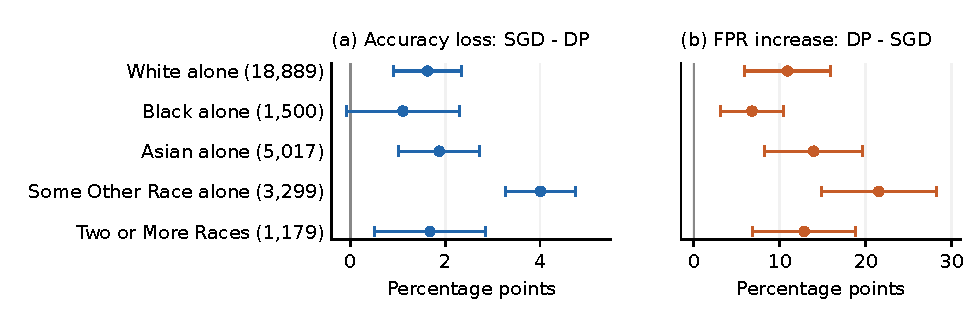
\includegraphics[width=\linewidth]{figures/racial_impact.pdf}
\caption{Paired DP1 changes, mean $\pm$ seed SD. Parentheses: development counts.
Headline races have $n\geq500$; smaller groups remain in detailed audits.}
\label{fig:impact}
\end{figure}

\newpage
\textbf{Fairness depends on the attribute and criterion.}
Sex separation falls $7.75\to5.03$ pp, while supported-race separation rises $16.72\to31.24$ pp
(both directions in 5/5 seeds). Black-alone versus Some Other Race-alone FPR (26.61\% vs 57.86\%)
drives DP1 race separation. Both sexes have higher FPR and lower accuracy despite closer sex parity.

\begin{table}[H]
\centering
\begin{tabular*}{\linewidth}{@{\extracolsep{\fill}}lrrrr@{}}
\toprule
 & \multicolumn{2}{c}{Sex} & \multicolumn{2}{c}{Supported race} \\
Gap (pp) & SGD & DP1 & SGD & DP1 \\
\midrule
Accuracy parity & $6.86\!\pm\!0.31$ & $6.17\!\pm\!0.48$ & $2.85\!\pm\!0.54$ & $4.91\!\pm\!0.48$ \\
Independence & $7.82\!\pm\!2.34$ & $6.45\!\pm\!1.26$ & $17.83\!\pm\!0.99$ & $25.26\!\pm\!1.07$ \\
Separation & $7.75\!\pm\!3.00$ & $5.03\!\pm\!0.71$ & $16.72\!\pm\!2.77$ & $31.24\!\pm\!1.44$ \\
Binary sufficiency & $9.29\!\pm\!0.46$ & $8.72\!\pm\!0.76$ & $4.64\!\pm\!0.95$ & $4.28\!\pm\!0.43$ \\
\midrule
\multicolumn{5}{l}{Overall accuracy (\%): SGD $77.42\pm0.55$; DP1 $75.52\pm0.34$} \\
\bottomrule
\end{tabular*}

\caption{Primary SGD versus DP1, mean $\pm$ seed SD. Smaller gaps indicate closer parity.}
\label{tab:fairness}
\end{table}
Gaps are accuracy/selection-rate ranges (accuracy parity/independence), the larger TPR/FPR range
(separation), and the larger PPV/NPV range (binary sufficiency, not score calibration).
Race sufficiency improves while the other race gaps worsen (Table~\ref{tab:fairness}).

\textbf{Clipping-associated loss.}
Accuracy is $77.42\pm0.55$\% for SGD, $77.57\pm0.41$\% for unclipped Poisson SGD,
$75.51\pm0.35$\% for clipped Poisson SGD, and $75.52\pm0.34$\% for DP1.
Clipped minus unclipped is $-2.06\pm0.48$ pp; DP1 minus clipped is $+0.005\pm0.051$ pp.
The reduction appears without noise, but DP uses fresh minibatches: this does not prove a sole cause
or that noise is irrelevant.

\textbf{Budget sensitivity and limitations.}
DP accuracy at $\eps=1,4,8$ is $75.517\pm0.343$, $75.550\pm0.334$, and $75.451\pm0.351$\%.
The mean span is 0.098 pp; $\eps=8$ is less accurate in all five $\eps=8$--$1$ pairs
($-0.066\pm0.042$ pp). Small effects here do not establish universal insensitivity or monotonicity.
Removing sensitive predictors reverses which sex loses more accuracy. One task/state/year, five seeds,
fixed $C=1$, and development-only evaluation limit generalization; tiny-group rates may be undefined.

\section{Remaining Work and Timeline}
\textbf{Nov.\ 19--24:} robustness checks, selected ten-seed runs, ACSIncome, and
$C\in\{0.5,1,2,5\}$ sensitivity if feasible (scaled noise/accounting).
\textbf{Nov.\ 24--30:} implement/evaluate LFR and EO with separate calibration and privacy assumptions.
\textbf{Dec.\ 1--4:} freeze choices, evaluate selected models on held-out test data, finalize trade-off figures.
\textbf{Dec.\ 5--7:} finalize report, presentation and reproducibility; deadline December 7, 2026.

\section{Changes from Original Proposal}
Primary inputs now include sex/race, with exclusion retained. Poisson/clipping ablations are new;
clipping-norm sensitivity is proposed. Original questions and LFR/EO objectives are unchanged.

\renewcommand{\refname}{References}
\begin{thebibliography}{4}
\setlength{\itemsep}{0pt}\setlength{\parskip}{0pt}
\bibitem{bagdasaryan2019} E.\ Bagdasaryan et al.\ \href{https://proceedings.neurips.cc/paper/2019/hash/fc0de4e0396fff257ea362983c2dda5a-Abstract.html}{Differential Privacy Has Disparate Impact on Model Accuracy}. \textit{NeurIPS}, 2019.
\bibitem{ding2021} F.\ Ding et al.\ \href{https://arxiv.org/abs/2108.04884}{Retiring Adult: New Datasets for Fair Machine Learning}. \textit{NeurIPS}, 2021.
\bibitem{hardt2016} M.\ Hardt et al.\ \href{https://arxiv.org/abs/1610.02413}{Equality of Opportunity in Supervised Learning}. \textit{NeurIPS}, 2016.
\bibitem{zemel2013} R.\ Zemel et al.\ \href{https://proceedings.mlr.press/v28/zemel13.html}{Learning Fair Representations}. \textit{ICML}, 2013.
\end{thebibliography}
\end{document}
